% 2014
% Maciej Szeptuch
% IIUWr

\documentclass[slidestop, compress, 10pt]{beamer}
\usetheme{Antibes}
\usecolortheme{lily}
\setbeamertemplate{footline}[frame number]

\usepackage[utf8]{inputenc}
\usepackage{polski}

\usepackage{multicol}
\usepackage{graphicx}

%% Kropka po numerze paragrafu, podparagrafu, itp.
\makeatletter
    \renewcommand\@seccntformat[1]{\csname the#1\endcsname.\quad}
    \renewcommand\numberline[1]{#1.\hskip0.7em}
\makeatother

%% Numeracja wzorów
\renewcommand{\theequation}{\arabic{section}.\arabic{equation}}

%% Plan przed każdą sekcją
\AtBeginSection[]
{
    \begin{frame}<beamer>
        \tableofcontents[currentsection]
    \end{frame}
}

%%%%%%%%%%%%%%%%%%%%%%%%%%%%%%%%%%%%%%%%%%%%%%%%%%%%%%%%%%%%%%%%%%%%%%%%%%%%%%%

\title{Symulacja ruchu drogowego}
\subtitle{na podstawie map z OpenStreetMap z użyciem technologii CUDA}
\author{Maciej Szeptuch}
\date{Wrocław, \today}

\begin{document}

% STRONA TYTUŁOWA
\begin{frame}
    \titlepage
\end{frame}

% PLAN
\begin{frame}
    \frametitle{Plan}
    \tableofcontents
\end{frame}

% Opis
\section{Opis}
    \begin{frame}
        \frametitle{Opis}
        \centering
        W czasie rzeczywistym chcę \textbf{symulować} i wizualizować ruch samochodów na danym \textbf{obszarze}.

        \begin{figure}
            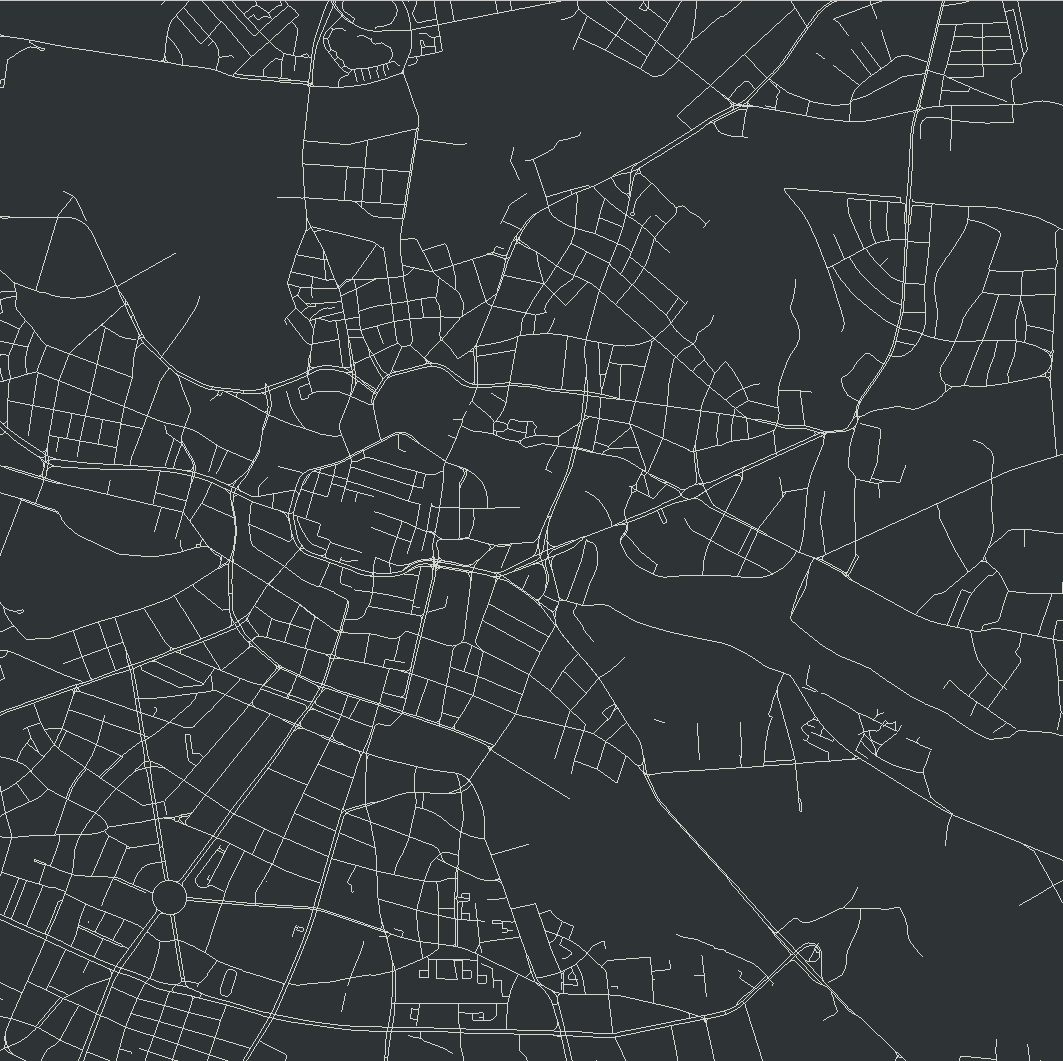
\includegraphics[width=100px]{trafficsim.png}
        \end{figure}

        \begin{block}{\textbf{rozmiar danych}}
            Wrocław zaimportowany z OpenStreetMap to $1.1 \cdot 10^5$ wierzchołków i $1.2 \cdot 10^5$ krawędzi. ($10$MB) \\
            Polska to $6 \cdot 10^6$ wierzchołków i $7 \cdot 10^6$ krawędzi. ($500$MB)
        \end{block}
    \end{frame}

% SYMULACJA
\section{Symulacja komputerowa}
    \begin{frame}
        \frametitle{Symulacja komputerowa}
        Za Wikipedią: "symulacja z wykorzystaniem modelu matematycznego, zapisanego w postaci programu komputerowego" \\
        Symulacje można podzielić ze względu na wiele różnych czynników. \\
        Najważniejsze: \\
        \begin{itemize}
            \item<2-> Przewidywalność zdarzeń
            \item<3-> "Modelowanie rzeczywistości"
            \item<4-> Sposób upływu czasu
            \item<5-> Poziom szczegółowości
        \end{itemize}
    \end{frame}

    \subsection{Przewidywalność zdarzeń}
        \begin{frame}
            \frametitle{Przewidywalność zdarzeń}
            \begin{itemize}
                \item<2-> \textbf{Stochastyczne} \\
                    Zdarzenia bazują na liczbach pseudolosowych.

                \item<3-> \textbf{Deterministyczne} \\
                    Wyniki symulacji zależą tylko od wejścia.
            \end{itemize}
        \end{frame}

    \subsection{"Model rzeczywistości"}
        \begin{frame}
            \frametitle{"Model rzeczywistości"}
            \begin{itemize}
                \item<2-> \textbf{Model matematyczny - równania różniczkowe, itp.} \\
                    Symulacja bazuje na pewnym model, obiekty są zazwyczaj reprezentowane sumarycznie przez ich właściwości. Symulacja polega zazwyczaj na obliczaniu odpowiednich równań do zmiany stanu symulacji.

                \item<3-> \textbf{Systemy agentów} \\
                    Każdy obiekt symulacji jest reprezentowany bezpośrednio przez tzw.\ agenta. Każdy agent ma swój stan, zbiór reguł i zachowań na podstawie których określa się jego stan w następnym kroku symulacji.
            \end{itemize}
        \end{frame}

    \subsection{Sposób upływu czasu}
        \begin{frame}
            \frametitle{Sposób upływu czasu}
            \begin{itemize}
                \item<2-> \textbf{Ciągły} \\
                    Na podstawie pewnych równań i/lub interpolacji obliczamy stan symulacji w \textit{dowolnym} momencie.

                \item<3-> \textbf{Dyskretny} \\
                    Co pewien stały, określony krok czasowy obliczamy kolejne stany symulacji.

                \item<4-> \textbf{Zdarzeniowy} \\
                    Dyskretny ze zmiennym krokiem czasowym. Stosowane w przypadkach gdy ważniejsza jest sekwencja zdarzeń niż upływ czasu.
            \end{itemize}
        \end{frame}

    \subsection{Poziom szczegółowości}
        \begin{frame}
            \frametitle{Poziom szczegółowości}
            \begin{itemize}
                \item<2-> \textbf{Mikroskopowy} \\
                    Określamy stan każdego obiektu z osobna (np.\ prędkość, pozycja samochodu).

                \item<3-> \textbf{Submikroskopowy} \\
                    Symulujemy "części" obiektów. W przypadku samochodów np.\ pojedyncze koła, hamulce itd.

                \item<4-> \textbf{Makroskopowy} \\
                    Dla każdego obiektu zbieramy sumaryczne informacje na podstawie których wykonujemy kroki symulacji (np.\ obciążenie - liczba / gęstość samochodów na drodze, skrzyżowaniu).

                \item<5-> \textbf{Mezoskopowy} \\
                    Hybryda powyższych podejść. Zbieramy obiekty w większe grupy i symulujemy je dokładnie jako jeden (wspólne zachowania).
            \end{itemize}
    \end{frame}

% PODOBNE PROJEKTY
\section{Podobne symulatory}
%% AORTA
    \subsection{AORTA}
    \begin{frame}
        \frametitle{Podobne symulatory - AORTA}
        \url{http://www.aorta-taffic.org} \\
        \begin{figure}
            
\includegraphics[width=200px]{aorta.png}
        \end{figure}
        Napisana w Skali. \\
        Z założenia "przyjazna" dla użytkownika, a mimo to zaawansowana. \\
        Pozwala importować mapy z OpenStreetMap i symulować na nich ruch. \\
        Model aukcyjny na skrzyżowaniach, \\
        Brak wsparcia dla GPU.
    \end{frame}

%% MATSIM
    \subsection{MATSIM}
    \begin{frame}
        \frametitle{Podobne symulatory - MATSIM}
        \url{http://www.matsim.org} \\
        \begin{figure}
            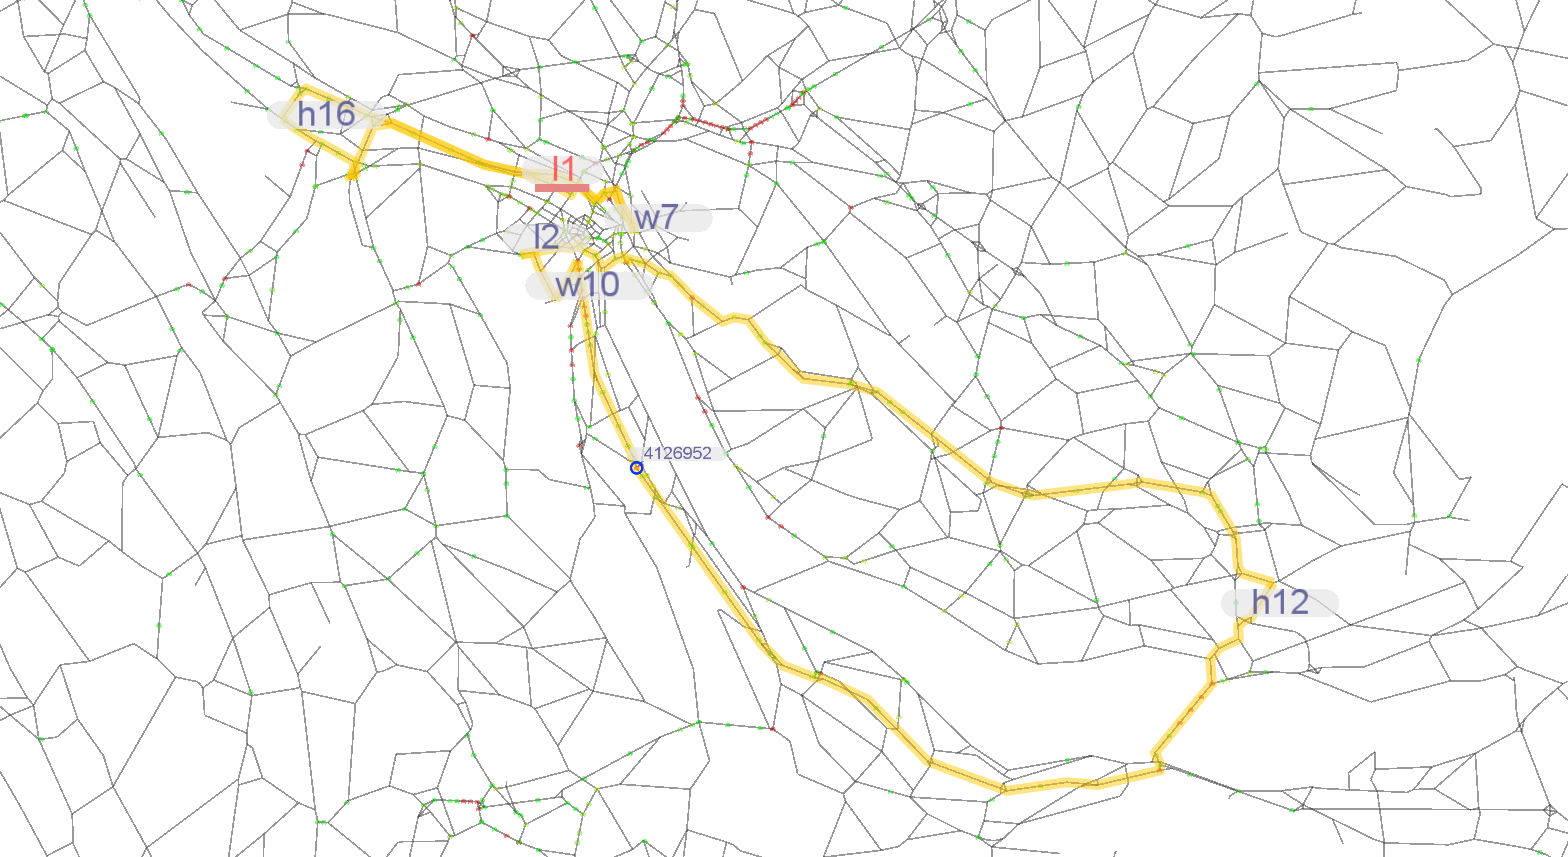
\includegraphics[width=200px]{matsim.png}
        \end{figure}
        Napisany w Javie. \\
        Rozbudowany framework pozwalający na wszelkiego rodzaju symulacje transportowe. \\
        Udostępnia także narzędzia do dokładnej analizy uzyskanych wyników. \\
        Brak wsparcia dla GPU.\ Eksperymentują z OpenCL. \\
        Domyślnie nie ma GUI - jeszcze.
    \end{frame}

%% SUMO
    \subsection{SUMO}
    \begin{frame}
        \frametitle{Podobne symulatory - SUMO}
        \url{http://sumo-sim.org} \\
        \begin{figure}
            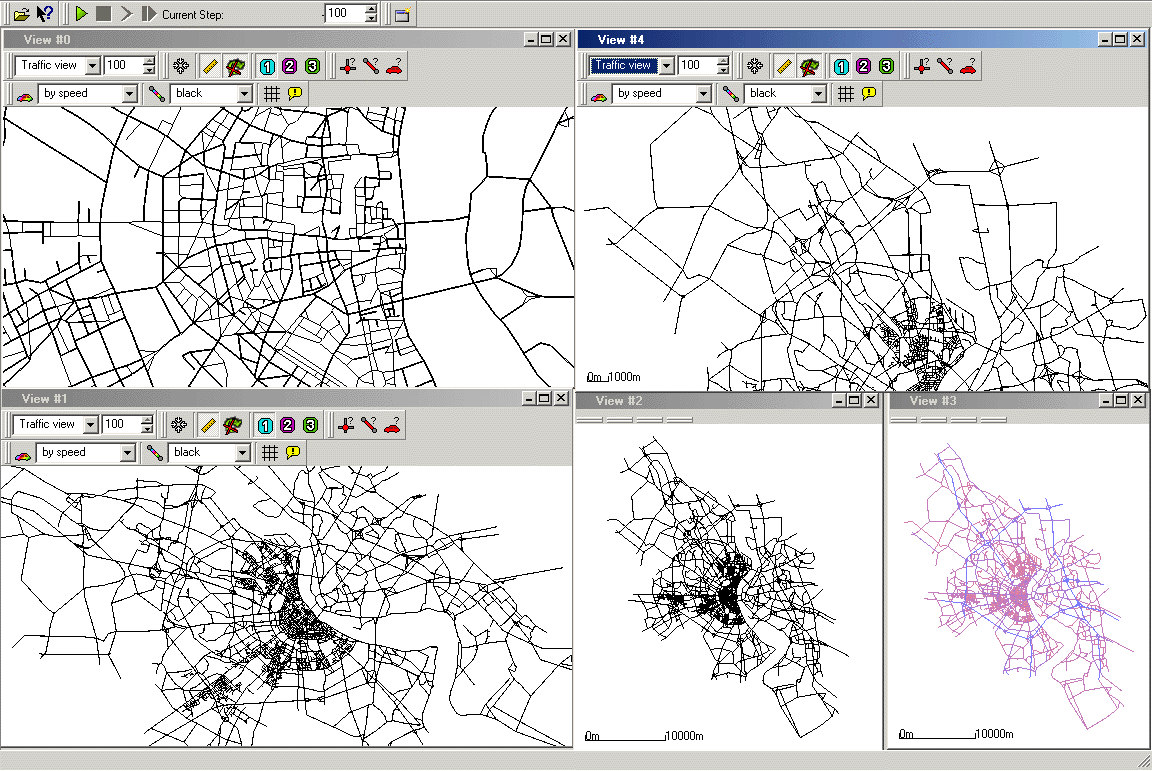
\includegraphics[width=200px]{sumo.png}
        \end{figure}
        Napisany w C++. \\
        Rozbudowany, przenośny. Nastawiony na wydajność. \\
        Pozwala na import danych z wielu różnych źródeł. \\
        System świateł \\
        Brak wsparcia dla GPU.
    \end{frame}

% ZAŁOŻENIA / UPROSZCZENIA
\section{Założenia / Uproszczenia}
    \begin{frame}
        Korzystam z systemu agentów przy mikroskopowej szczegółowości i stałym dyskretnym kroku czasowym. Daje mi to możliwość dokładnego symulowania, a zarazem pozwala na ciekawą wizualizację ruchu samochodów na mapie.
        \pause \\
        Stosuje pewne założenia i uproszczenia żeby ułatwić sobie życie.
        \begin{itemize}
            \item Spójny graf,
            \item Bardzo prosta fizyka samochodów (jedzie z określoną prędkością, hamuje w miejscu, itp.),
            \item Każdy samochód taki sam,
            \item Wszystkie skrzyżowania równorzędne.
        \end{itemize}

        \pause
        W miarę możliwości, jak wszystko będzie bezproblemowo działać planuje jeszcze parę usprawnień.
        \begin{itemize}
            \item Bardziej rzeczywista fizyka samochodów,
            \item Możliwość ręcznego dodawania samochodów,
            \item GUI do podglądania trasy konkretnego samochodu.
            \item Światła na skrzyżowaniach,
        \end{itemize}
    \end{frame}

% MAPA
\section{Mapa}

%% OPENSTREETMAP
    \subsection{OpenStreetMap}
        \begin{frame}
            \frametitle{OpenStreetMap}
            \begin{figure}
                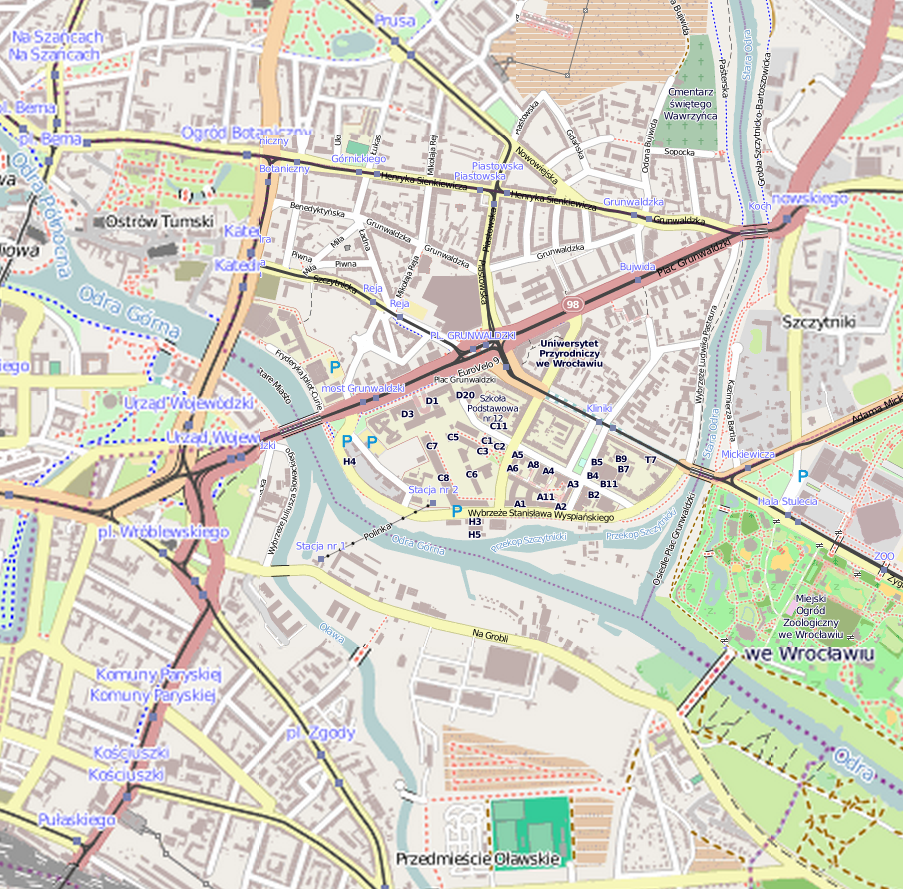
\includegraphics[width=200px]{osm.png}
            \end{figure}
        \end{frame}
        \begin{frame}[allowframebreaks]
            \frametitle{OpenStreetMap}
            \url{http://openstreetmap.org} \\
            ~ \\
            Darmowa mapa całej kuli ziemskiej, którą może współtworzyć każdy (coś jak Wikipedia tylko dla map). \\
            ~ \\
            Udostępnia wszystkie zebrane dane na otwartej licencji Open Database License. \\
            ~ \\
            Dane od użytkowników są gromadzone w bazie danych. Istnieje możliwość pobierania dowolnych obszarów w formatach XML lub osm.pbf (google-protobuf). \\
            ~ \\
            Aktualny rozmiar bazy całej planety to 32GB w formie skompresowanego bzipem XML, lub 23GB w protobuf.
            ~ \\
            ~ \\
            ~ \\
            \begin{block}{format danych}
                Dane z OSM są zorganizowane w cztery główne typy:
                \begin{itemize}
                    \item \textbf{Węzły}    - punkty z pozycją geograficzną
                    \item \textbf{Drogi}    - listy węzłów reprezentujące nie tylko drogi ale także wszystkie wielokąty występujące na mapie
                    \item \textbf{Relacje}  - grupy węzłów, dróg i innych relacji
                    \item \textbf{Tagi}     - pary klucz=wartość, każdy z trzech powyższych typów może posiadać dowolną liczbę tagów
                \end{itemize}
            \end{block}
        \end{frame}

%% GRAF
    \subsection{Graf}
        \begin{frame}
            \frametitle{Graf}
            \begin{itemize}
                \item W bazie OSM znajduje się bardzo dużo wszelkiego rodzaju informacji (drogi samochodowe, rowerowe, piesze, budynki, znaki, itd.).
                \item<2-> Z założeń chcę mieć spójny graf.
                \item<3-> Jedyne co mnie interesuje to drogi, po których mogą jeździć samochody.
                \item<4-> Potrzebuje także dodatkowych informacji typu czy droga jest jednokierunkowa, liczby pasów, ograniczeń prędkości.
                \item<5-> Pozwala to znacząco zmniejszyć wielkość grafu.
            \end{itemize}

            \only<6->{\begin{block}{struktura grafu}
                Ostatecznie wierzchołki, które reprezentują skrzyżowania, nie przechowują żadnych dodatkowych informacji, natomiast krawędzie reprezentujące drogi zawierają informacje o liczbie pasów i ograniczeniach prędkości.
            \end{block}}
        \end{frame}

% CUDA
\section{CUDA}
    \begin{frame}
        \frametitle{Symulacja użyciem CUDA}
        Ogólny model dosyć prosty. Symulujemy agentów na osobnych wątkach, być może ich grupując. \\
        \only<2->{\textbf{Problemy?} \\}
        \only<3->{Trzeba jakoś podzielić agentów na wątki. \\}
        \only<4->{Podział po wątku na agenta - nieoptymalny. \\}
        \only<5->{Każdy samochód potrzebuje informacji o okolicznych aby określić co może dalej zrobić. \\}
        \only<6->{Dużo lepszym pomysłem wydaje się przydzielać wątkom grupy samochodów w postaci na przykład spójnego kawałka mapy. \\}
        \only<7->{Pozwala to optymalizować użycie pamięci a zarazem upraszcza wyszukiwanie kolizji bo już z góry wiemy kto jest w pobliżu. \\}
    \end{frame}

    \begin{frame}
        \frametitle{Symulacja użyciem CUDA}
        Gdzie trzymamy dane symulacji? \\
        \begin{itemize}
            \item<2-> Na CPU \\
                Najwygodniej, prosto debugować. Można wizualizować dowolnym sposobem. \\
                Dużo kopiowania pomiędzy kartą a procesorem.

            \item<3-> Na GPU \\
                Szybko. Brak narzutów ciągłego kopiowania danych. \\
                Możemy wizualizować w OpenGL. \\
                Nie tak prosto z debugowaniem, badaniem stanu symulacji - można kopiować dane spowrotem do RAMu
        \end{itemize}
    \end{frame}

\section{QA}
    \begin{frame}
        \frametitle{Pytania?}
        \centering
        ~ \\
        ~ \\
        ~ \\
        ~ \\
        ~ \\
        ~ \\
        ~ \\
        Pytania / Uwagi ?
    \end{frame}

\end{document}
